\title[Graph Analytics]{\textbf{Graph Analtyics}}

\begin{document}

\newcommand{\Path}{\ell}
\newcommand{\Diam}{\mathit{diam}}

\begin{frame}
\titlepage

{\footnotesize
Acknowledgment for some slides: Mark Jelasity, Sebastian Ahnert, Lada Adamic, Albert Diaz Guilera, Bill Howe
}

\invisible{
\nobibliography*{../references}
}

\end{frame}

\begin{frame}[shrink]{Contents}
\tableofcontents
\end{frame}

%%%%%%%%%%%%%%%%%%%%%%%%%%%%%%%%%%%%%%%%%%%%%%%%%%%%%%%%%%%%%%%%%%%%%%%%

\section{Introduction}

\begin{frame}{Introduction}

\begin{block}{What these structures have in common?}

\begin{columns}
\begin{column}{0.5\textwidth}
\BI
\item World Wide Web
\item Internet
\item Movie actor collaborations
\item Science collaborations
\item Citations of papers
\item Sexual relationships
\EI
\end{column}
\begin{column}{0.5\textwidth}
\BI
\item Food webs
\item Facebook \& Linkedin
\item Co-occurrence of words
\item Your brain
\item The power network of USA
\item Protein folding
\EI
\end{column}
\end{columns}
\end{block}

\pause
\bigskip
\BI
\item They can be described as graphs
\pause
\item They all show similar features!
\EI

\end{frame}


\begin{frame}{Complex network research}

\BIL
\item Rapidly increasing interest over the last decade, since much more network data available now
\item Multidisciplinary research 
  \BI
  \item Physics
  \item Biology
  \item Sociology
  \item Mathematics
  \item Epidemiology
  \item \ldots
  \EI
\item Strong implications for Computer Science
\BI
\item Robustness of networks
\item Efficiency: function of networks depends on their structure
\item Design and engineering
\EI
\EIL
\end{frame}

\begin{frame}{Complex network research}

\begin{columns}
\begin{column}{0.4\textwidth}
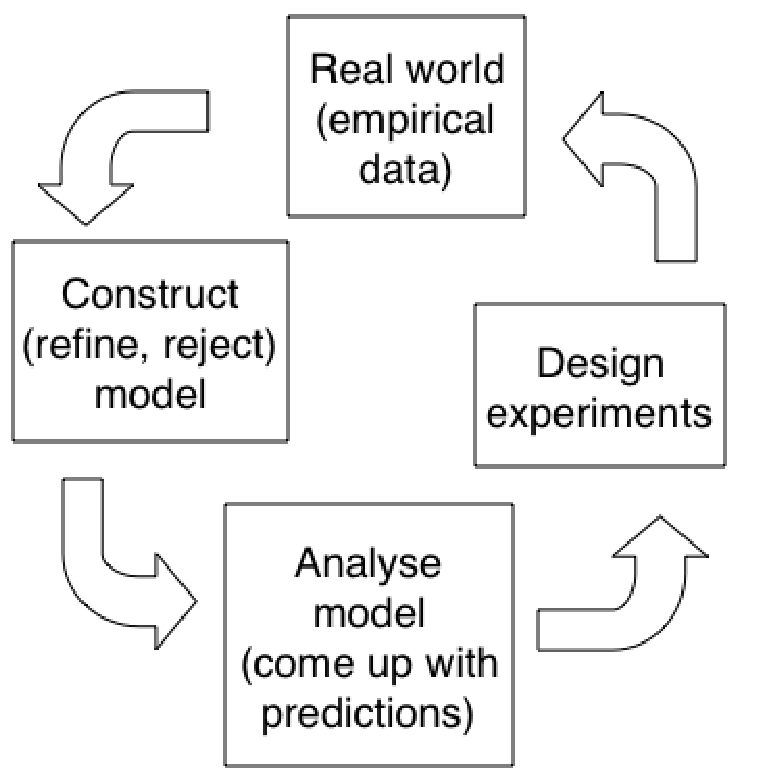
\includegraphics[width=\textwidth]{figs/08/experimental}
\end{column}
\begin{column}{0.6\textwidth}
\BIL
\item Complex networks is a branch of physics
\item Empirical science: loop of modeling and observation
\item Models are models
\BI
\item Explain some aspects
\item Don't explain other aspects
\EI
\item Has a lot to do with condensed matter physics
\EIL
\end{column}
\end{columns}


\end{frame}

\section{Topological properties}

\subsection{Degree statistics}

\begin{frame}{Degree statistics (1)}

\begin{definition}[Degree]
\BI
\item The \alert{degree} $k_i$ of node $i$ is the number of edges the node has to other nodes
\item In this lecture, we will only consider undirected graphs
\item Called \alert{local centrality} in social network analysis
\item Measures how important is a node with respect to its neighbors
\EI
\end{definition}	

\begin{figure}
	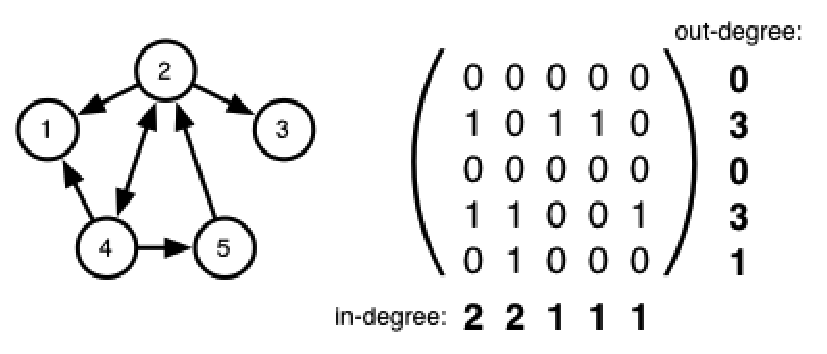
\includegraphics[width=0.75\textwidth]{figs/08/degree}
\end{figure}


\end{frame}

\begin{frame}{Degree statistics (2)}

\begin{definition}[Degree distribution]
\BI
\item The average degree of a graph $G=(V,E)$ is $\langle k \rangle = \frac{|E|}{|V|}$ 
\item $P(k)$ is the probability that a random node has degree $k$
\item The probability distribution gives an idea of the spread in the number of links the nodes have
\EI
\end{definition}

\begin{figure}
	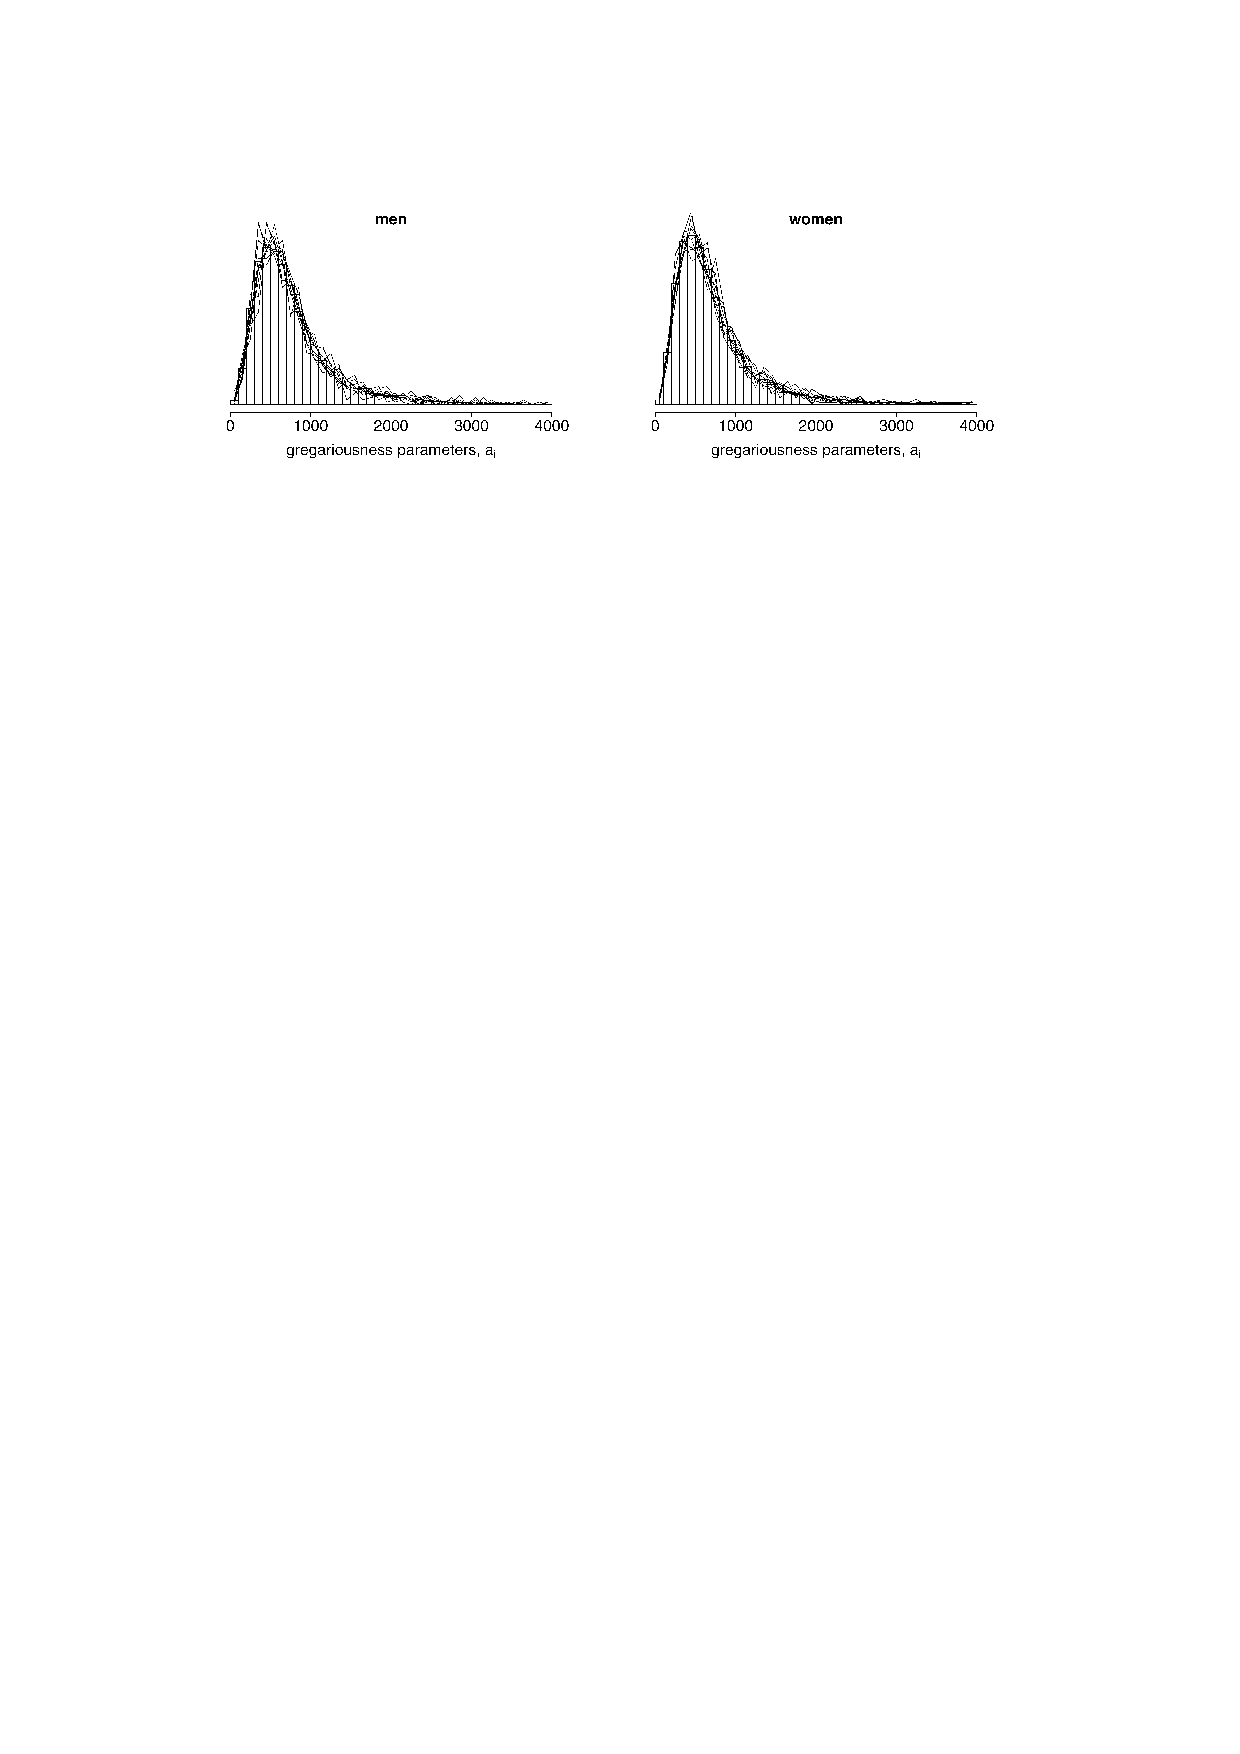
\includegraphics[width=0.8\textwidth]{figs/08/degreedist}
\end{figure}
	
\note{
Tian ZHENG, Matthew J. SALGANIK, and Andrew GELMAN. How Many People Do You Know in Prison?: Using
Overdispersion in Count Data to Estimate Social Structure in Networks. In Journal of the American Statistical Association, 2006
}	
	
\end{frame}


\begin{frame}{Degree statistics (3) - Exponential distribution}

\BI
\item Exponential distribution:
\[
  P(k) = c x^k
\]
for some $c$, for some $x<1$
\item A \alert{random graph} has exponential distribution 
\item Best seen on a log scale
\EI
		
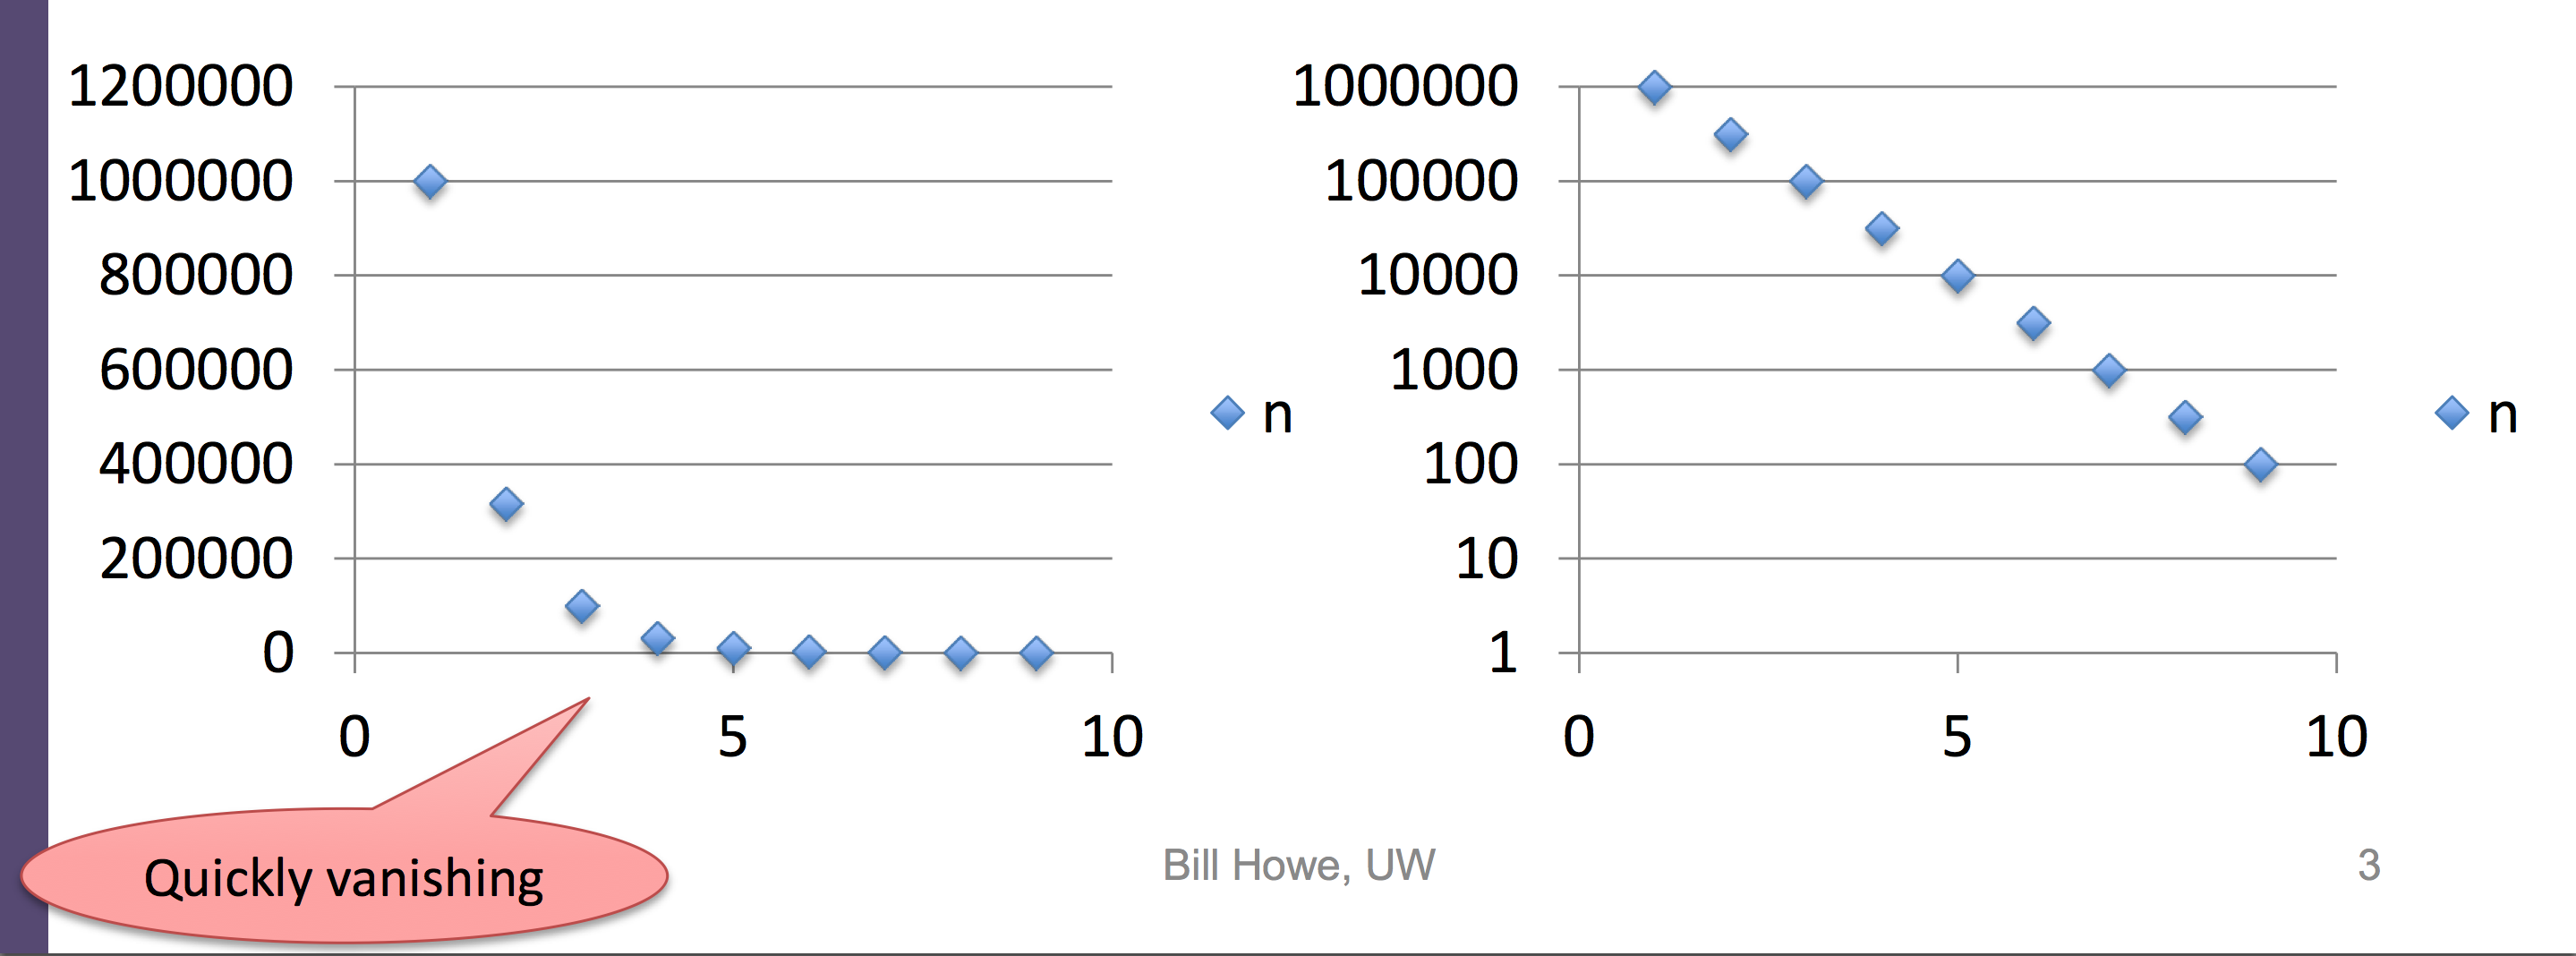
\includegraphics[width=1.0\textwidth]{figs/xx/degree1}
		
\end{frame}

\begin{frame}{Degree statistics (4) - Zipf distribution}

\BI
\item Zipf distribution:
\[
  P(k) \approx k^{-\lambda}
\]
\item Human-generated data has Zipf distribution: letters in alphabet, words in vocabulary, etc.
\item Best seen on a log-log scale
\EI
		
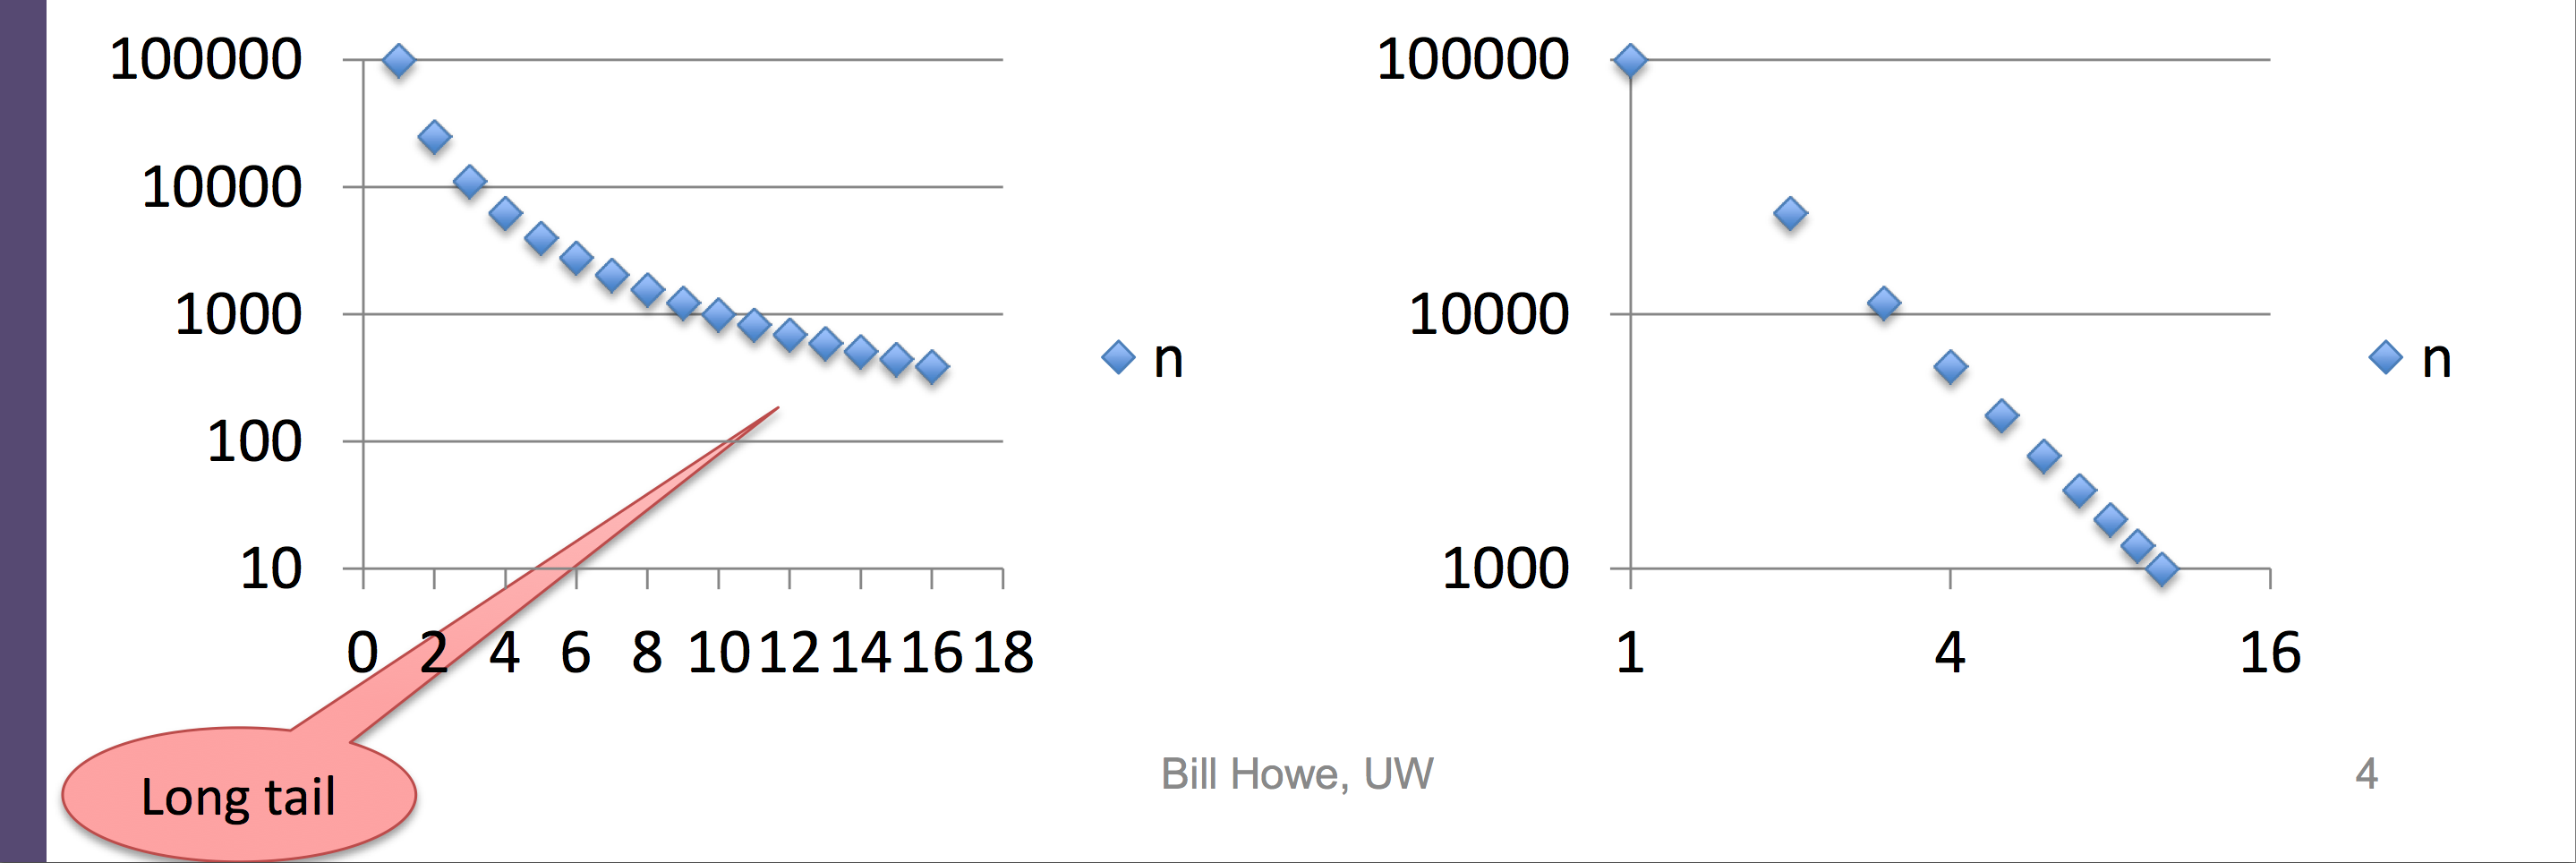
\includegraphics[width=1.0\textwidth]{figs/xx/degree2}
		
\end{frame}

\begin{frame}{Degree statistics (4) - Zipf distribution}
\begin{figure}
	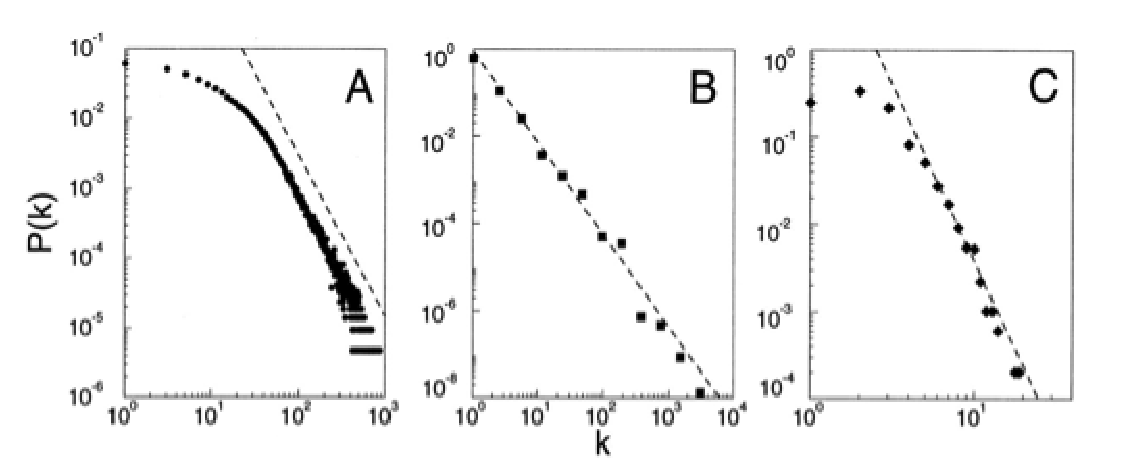
\includegraphics[width=0.9\textwidth]{figs/08/threeex}
	\caption{Real network degree distributions: from left to right, Actors, WWW, Power grid}
\end{figure}
\end{frame}



\subsection{Distance statistics}

\begin{frame}{Distance statistics (1)}

\begin{definition}[Path length]
The \alert{path length} $d(i,j)$, or \alert{goedesic distance}, between two nodes $i$ and $j$ is the length
of the shortest path connecting them. 
\end{definition}

\begin{figure}
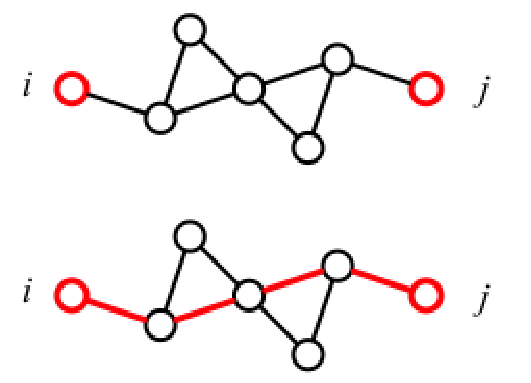
\includegraphics[width=0.6\textwidth]{figs/08/distance}
\end{figure}

\end{frame}

\begin{frame}{Distance statistics (2)}
	
\begin{definition}[Average path length]
The \alert{average path length} of a connected graph $G=(V,E)$ is defined as:
\[
  \Path(G) = \frac{1}{|V|(|V|-1)} \sum_{i,j \in V, i \neq j} d(i,j)
\]
\end{definition}

\begin{figure}
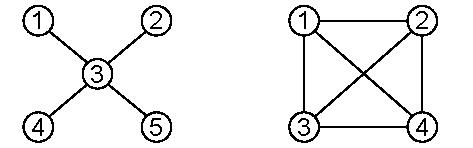
\includegraphics[width=0.6\textwidth]{figs/08/diameter}
\caption{(a) $\Path(G) = (4 \cdot ((2+2+2+1)/8) + 1)/5=1.6$. (b) $\Path(G) = 1$}
\end{figure}

\end{frame}


\begin{frame}{Distance statistics (3)}

\begin{definition}[Diameter]
The \alert{diameter} is the maximal shortest path between any two vertices:
\[
  \Diam(G) = \max \{ d(i,j) : i,j \in V \}
\]
\end{definition}

\begin{figure}
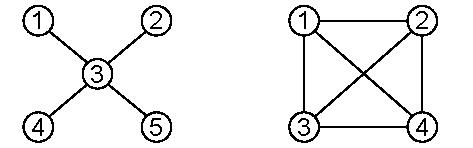
\includegraphics[width=0.6\textwidth]{figs/08/diameter}
\caption{(a) $\Diam(G) = 2$. (b) $\Diam(G) = 1$}
\end{figure}

\end{frame}

\subsection{Clustering coefficient}

\begin{frame}{Clustering coefficient (1)}

\begin{definition}[Induced graphs]
The subgraph $G_i=(V_i, E_i)$ \alert{induced} by node $i$ over a graph $G=(V,E)$ 
  is given by the neighbors of $i$ and the edges linking them:
  \begin{align*}
	 V_i &= \{ j : j \in V \wedge (i,j) \in E \} \\
	 E_i &= \{ (i,j) : i,j \in V_i \wedge (i,j) \in E \} 
  \end{align*}
\end{definition}

\bigskip
\begin{overprint}
\onslide<1|handout:0>
\begin{figure}
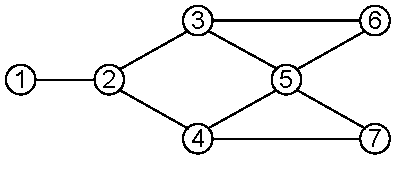
\includegraphics[width=0.7\textwidth]{figs/08/induced1}
\end{figure}
\onslide<2|handout:1>
\begin{figure}
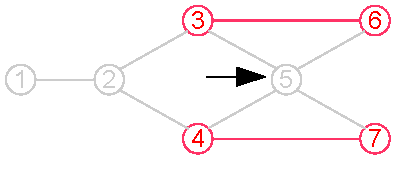
\includegraphics[width=0.7\textwidth]{figs/08/induced2}
\end{figure}
\end{overprint}
\end{frame}

\begin{frame}{Clustering coefficient (2)}

\begin{definition}[Local clustering coefficient]
The \alert{local clustering coefficient} of node $i$ in graph $G$ is the
  ratio between the size of $|E_i|$ and the number of all potential edges
  that link two nodes in $V_i$:
  \[
     CC(G,i) = \frac{|E_i|}{|V_i|(|V_i|-1)/2} = \frac{2|E_i|}{|V_i|(|V_i|-1)}
  \]
\end{definition}

\begin{figure}
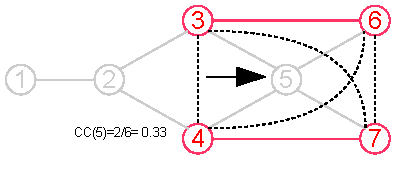
\includegraphics[width=0.7\textwidth]{figs/08/induced3}
\end{figure}

\end{frame}

\begin{frame}{Clustering coefficient (3)}

\begin{definition}[Clustering coefficient]

The \alert{clustering coefficient} of graph $G$ is the average over the local 
  clustering coefficient of all nodes in the graph
  \[
     CC(G) = \frac{1}{N} \sum_{i \in V} CC(G,i)
  \]
\end{definition}

\begin{columns}
	\begin{column}{0.35\textwidth}
		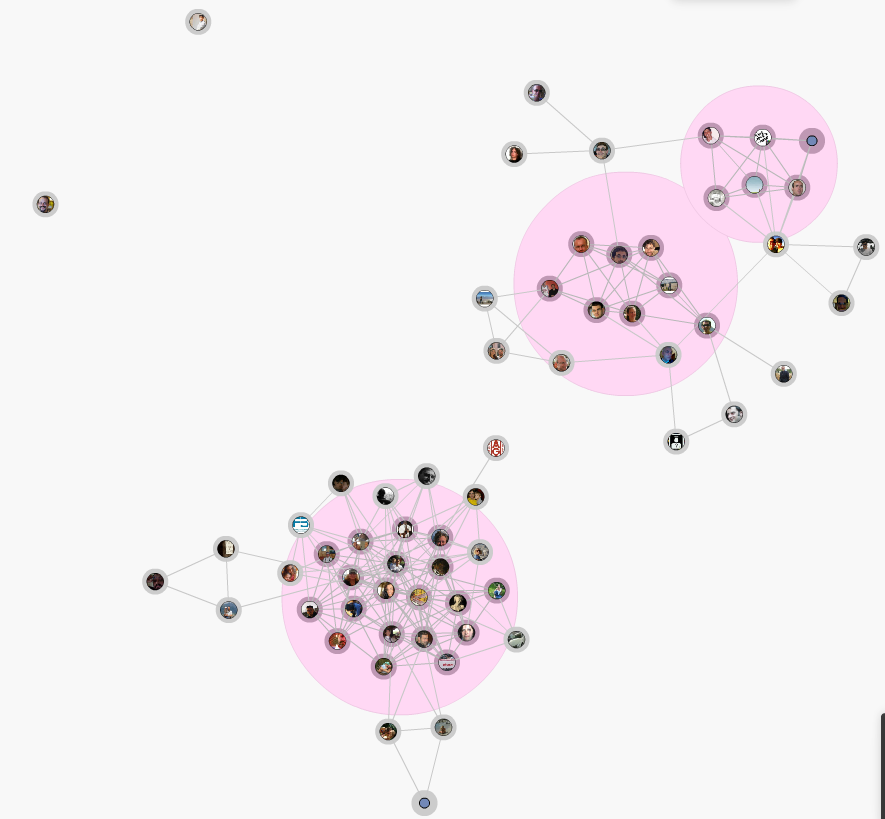
\includegraphics[width=\textwidth]{figs/08/facebook}
	\end{column}
	\begin{column}{0.65\textwidth}
		\BI
		\item Facebook clustering coefficient 0.16
		\EI
	\end{column}
\end{columns}
\end{frame}

\subsection{Connectivity coefficient}

\begin{frame}{Connectivity coefficient}

\begin{definition}[Connectivity coefficient]
Minimum number of vertices you need to remove that will disconnect the graph.
\end{definition}


\begin{columns}
	\begin{column}{0.5\textwidth}
		\BI
		\item What is the connectivity coefficient of this graph?
		\item May depend on what is meant by “connectivity”
		\BI
		\item Strong connectivity
		\item Weak connectivity
		\EI
		\item Why might you want to compute the connectivity coefficient?
		\EI
	\end{column}
	\begin{column}{0.5\textwidth}
		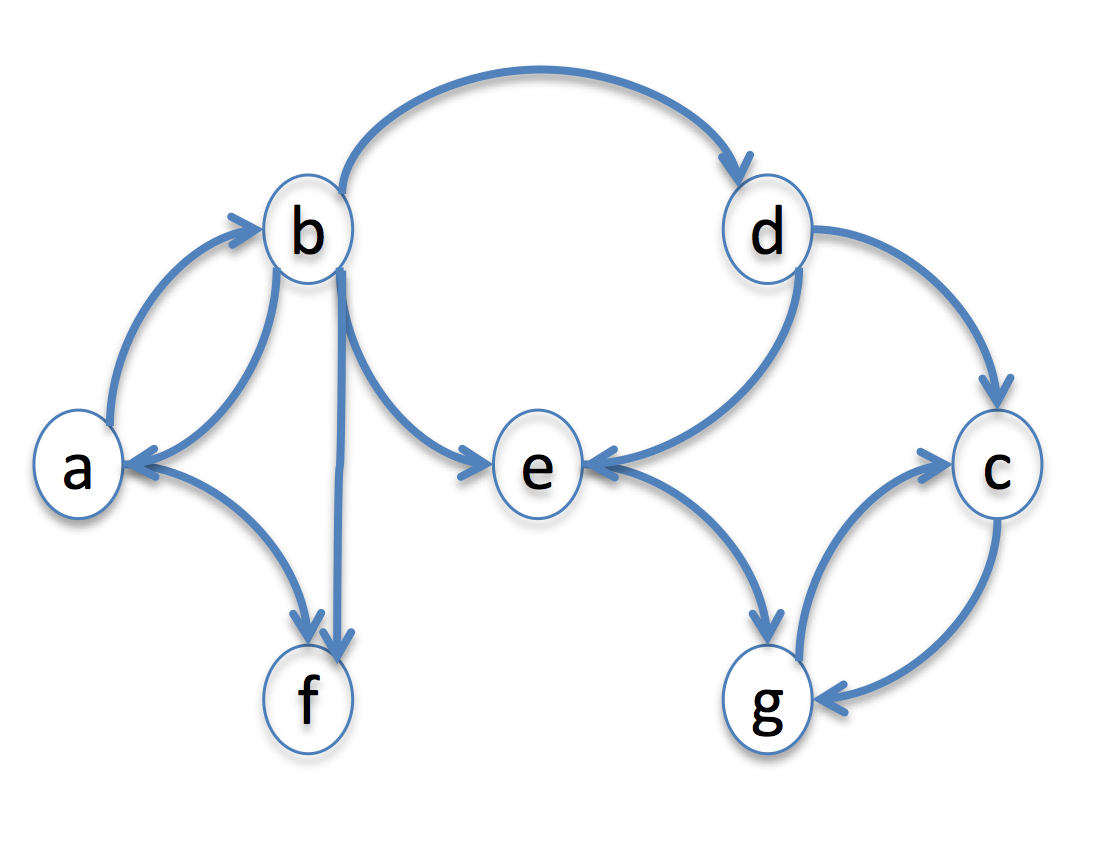
\includegraphics[width=\textwidth]{figs/xx/connectivity.png}
	\end{column}
\end{columns}



	

\end{frame}

\subsection{Centrality measures}


\begin{frame}{Centrality measures}

\begin{definition}[Centrality]
The (relative) \alert{importance} of a vertex with respect to its position in the graph
\end{definition}

\begin{columns}
	\begin{column}{0.5\textwidth}
		\BI
			\item \alert{Closeness Centrality} of a vertex $v$: \\
			Average length of all its shortest paths originating from $v$
			\item \alert{Betweenness Centrality} of a vertex $v$: \\
			the fraction of all shortest paths that pass through $v$
		\EI
	\end{column}
	\begin{column}{0.5\textwidth}
		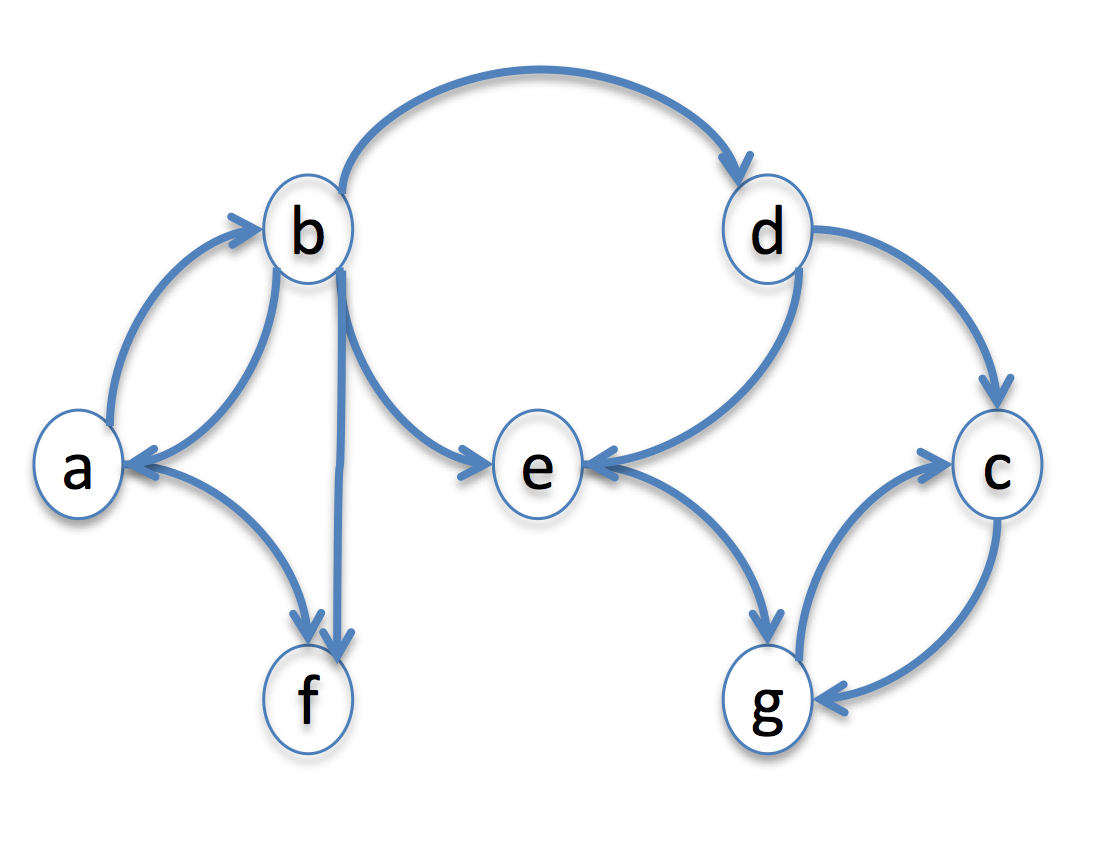
\includegraphics[width=\textwidth]{figs/xx/connectivity.png}
	\end{column}
\end{columns}


\end{frame}


\begin{frame}{Centrality measures}

\begin{definition}[Degree Centrality]
\alert{Degree centrality} of a vertex $v$: $d(v)/|E|$
\end{definition}

\begin{columns}
	\begin{column}{0.5\textwidth}
		\BI
			\item “Important” nodes are those with high degree
			\item But: say we both have 5 friends
			\BI
			\item We have the same degree centrality
			\item But what if your 5 friends are Barack Obama, Larry Page, Bill Gates, the Dalai Lama, and Oprah Winfrey?
			\item Shouldn’t you be considered more “important?”
			\EI
		\EI
	\end{column}
	\begin{column}{0.5\textwidth}
		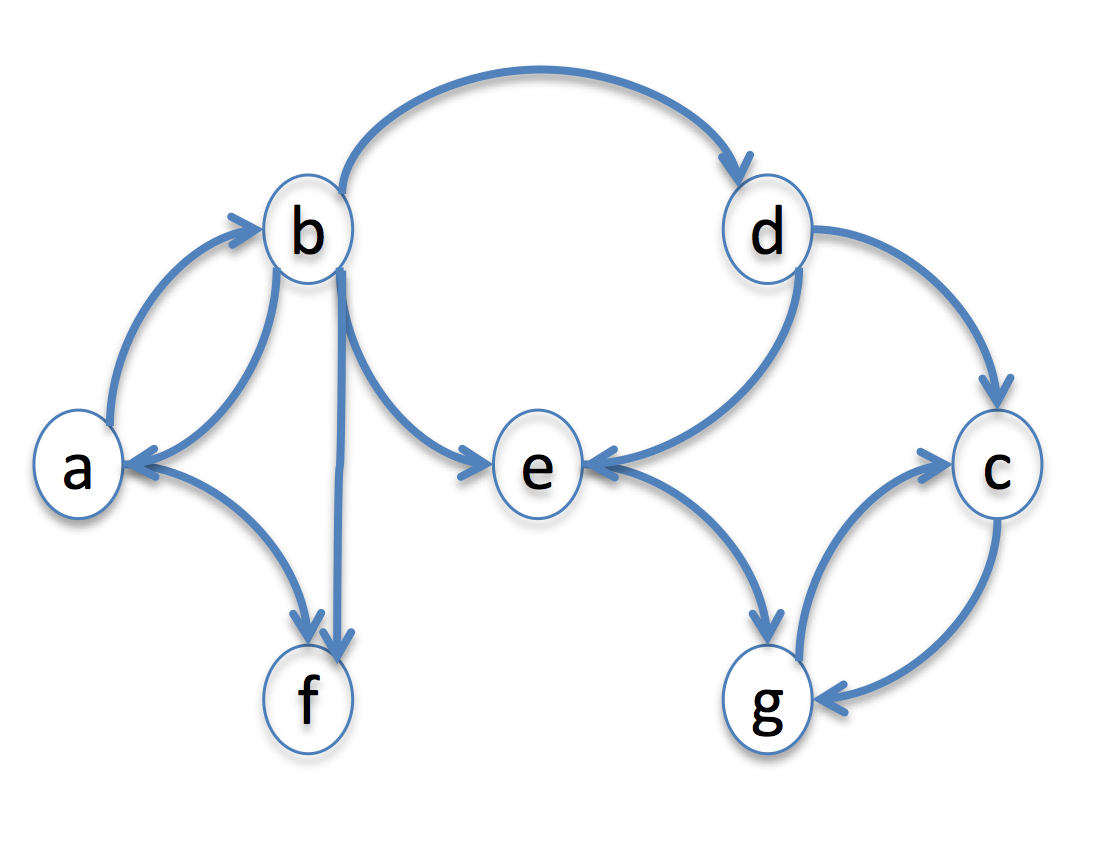
\includegraphics[width=\textwidth]{figs/xx/connectivity.png}
	\end{column}
\end{columns}

\end{frame}


\begin{frame}{EigenVector Centrality (PageRank)}
	
Basic idea (oversimplified):
\begin{Procedure}
\While{not converged}{
  \ForEach{vertex $v$}{
  	$\mathit{rank}(v) =$ sum of ranks from incoming edges
  }
}	
\end{Procedure}


Some problems:
\BI
\item If a page with millions of outgoing links links to me, that’s less valuable than a page with only a few outgoing links.
\item Written like this, it does not converge
\item  If I’m 27 hops away from Barack Obama, he shouldn’t really influence my rank. 
\EI

We need a \emph{damping factor}!

\end{frame}

\begin{frame}{EigenVector Centrality (PageRank)}
\begin{Procedure}
\While{not converged}{
  \ForEach{vertex $v$}{
  	$\mathit{rank}(v) = \frac{1-d}{N} + d \sum_{\forall (v,u) \in E} \frac{\mathit{rank}(u)}{d_{\mathit{out}}}(u)$ 
  }
}	
\end{Procedure}
where:
\BI
\item $\mathit{rank}(v)$ is the page rank (centrality) of $v$
\item $d_{\mathit{out}}(u)$ is the out-degree of $v$
\item $N$ is the total number of nodes	
\item $d$ is the dumping factor ($0 < d < 1$)
\EI
\end{frame}

\begin{frame}{The Milgram Small-World Experiment}

Milgram's experiment (1967):

Given a target individual and a particular property, pass the message to a 
person you correspond with who is “closest” to the target.

\begin{figure}
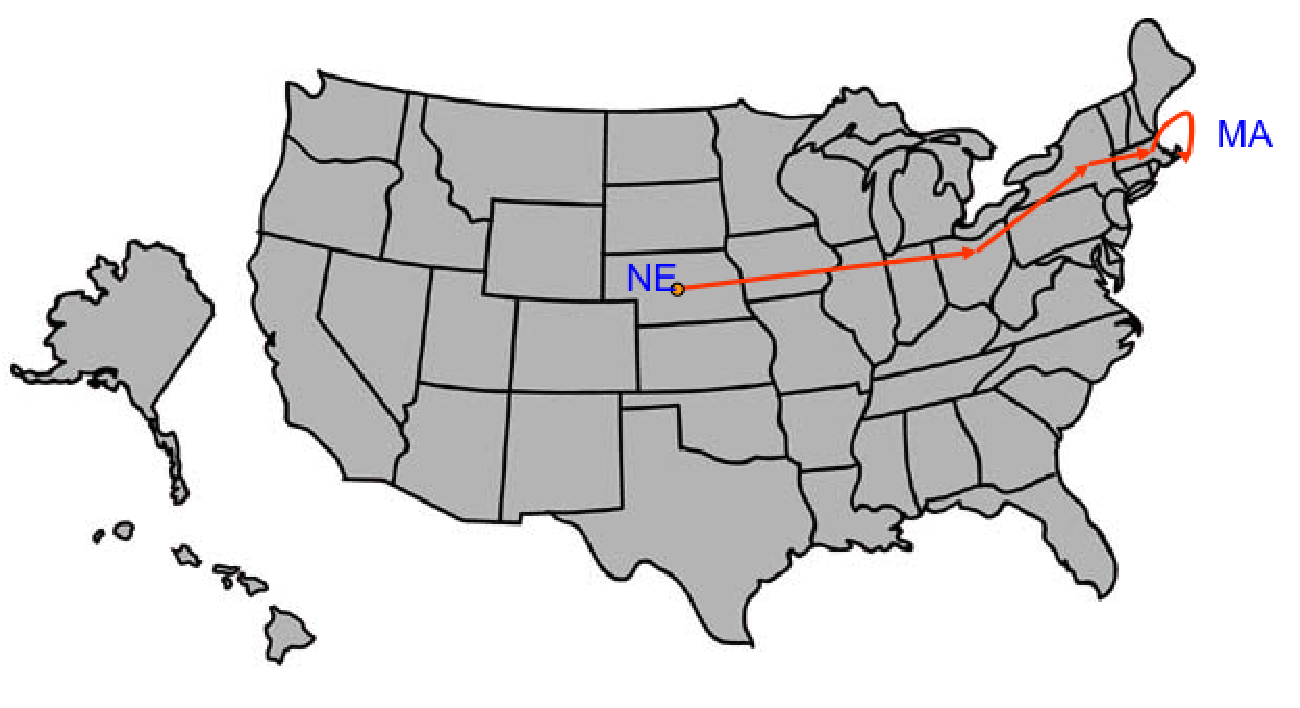
\includegraphics[width=0.8\textwidth]{figs/08/milgram}
\end{figure}
	
\end{frame}

\begin{frame}{The Milgram Small-World Experiment}
	
\structure{Some facts}:

\BI
\item Target person worked in Boston as a stockbroker.
\item 296 senders from Boston and Omaha.
\item 20\% of senders reached target.
\item Average path length = 6.5.
\EI

\bigskip
\structure{“Six degrees of separation”}:

\BI
\item It's a small world after all!
\item Kevin-Bacon game
\item Erd\"os number
\EI

\end{frame}

\begin{frame}{Six Degrees and Popular Culture}

\begin{columns}
\begin{column}{0.65\textwidth}
\begin{block}{“Everything is Different”\\ Frigyes Karinthy, 1929}
\begin{quote}
{\footnotesize
A fascinating game grew out of this discussion. One of us suggested performing
the following experiment to prove that the population of the Earth is closer
together now than they have ever been before. We should select any person from
the 1.5 billion inhabitants of the Earth—anyone, anywhere at all. He bet us
that, using no more than five individuals, one of whom is a personal
acquaintance, he could contact the selected individual using nothing except
the network of personal acquaintances.}
\end{quote}
\end{block}
\end{column}
\begin{column}{0.35\textwidth}
	
\includegraphics[width=\textwidth]{figs/08/sixdegrees}
\end{column}
\end{columns}


\note{
\BI
\item Frigyes Karinthy is an Hungarian author.
\item The original ideas come out from Guglielmo Marconi's Nobel lecture - but
 I was not able to find such link in the speech
\item Six Degrees of Separation is a 1993 film drama featuring Will Smith, Donald Sutherland and Stockard Channing
\item Will Smith and Charlie Chaplin have a distance of $3$, through Jack Lemmon and Hank Mann
\EI
}

\end{frame}

%%%%%%%%%%%%%%%%%%%%%%%%%%%%%%%%%%%%%%%%%%%%%%%%%%%%%%%%%%%%%%%%%%%%%%%%

\section{Frameworks for Big Graph Analytics}


\begin{frame}{(Really) Big Graphs}

\begin{columns}[T]
\begin{column}{0.6\textwidth}
\BI
\item Social scale:\\
1 billion vertices, 100 billion edges
\item Web scale:\\
50 billion vertices, 1 trillion edges
\item Brain scale:\\
100 billion vertices, 100 trillion edges	
\EI
\begin{center}
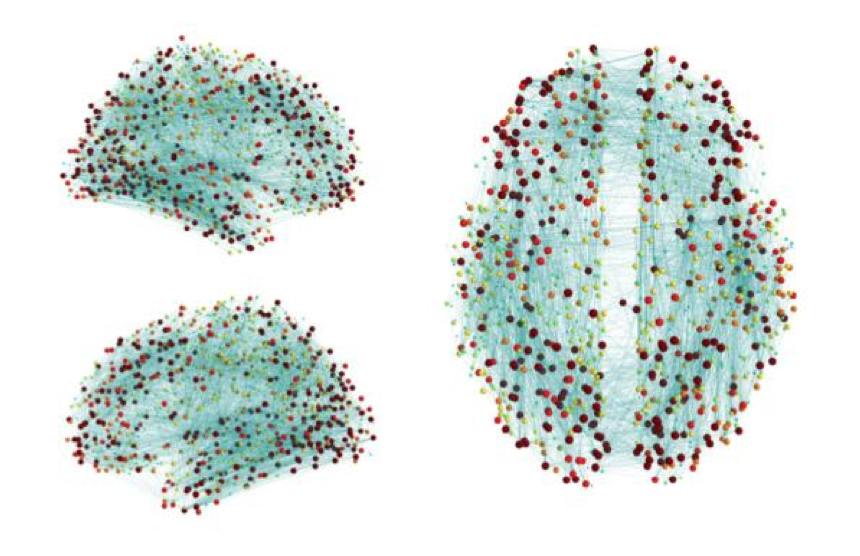
\includegraphics[width=0.80\textwidth]{figs/xx/brain.png}\\	
\end{center}
\end{column}
\begin{column}{0.4\textwidth}
\begin{center}
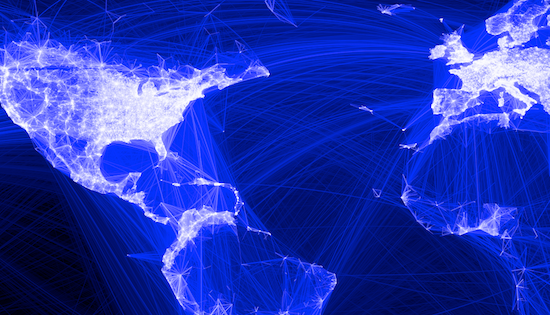
\includegraphics[width=0.80\textwidth]{figs/xx/fb.png}\\	
~\\
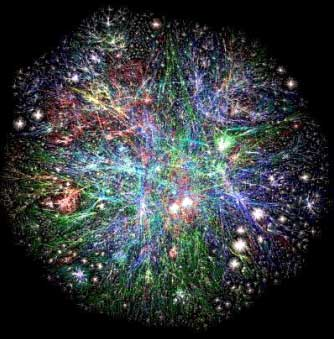
\includegraphics[width=0.80\textwidth]{figs/xx/web.jpg}
\end{center}
\end{column}
\end{columns}
	
\end{frame}

	
	
\begin{frame}{Example: Map Reduce for PageRank}	

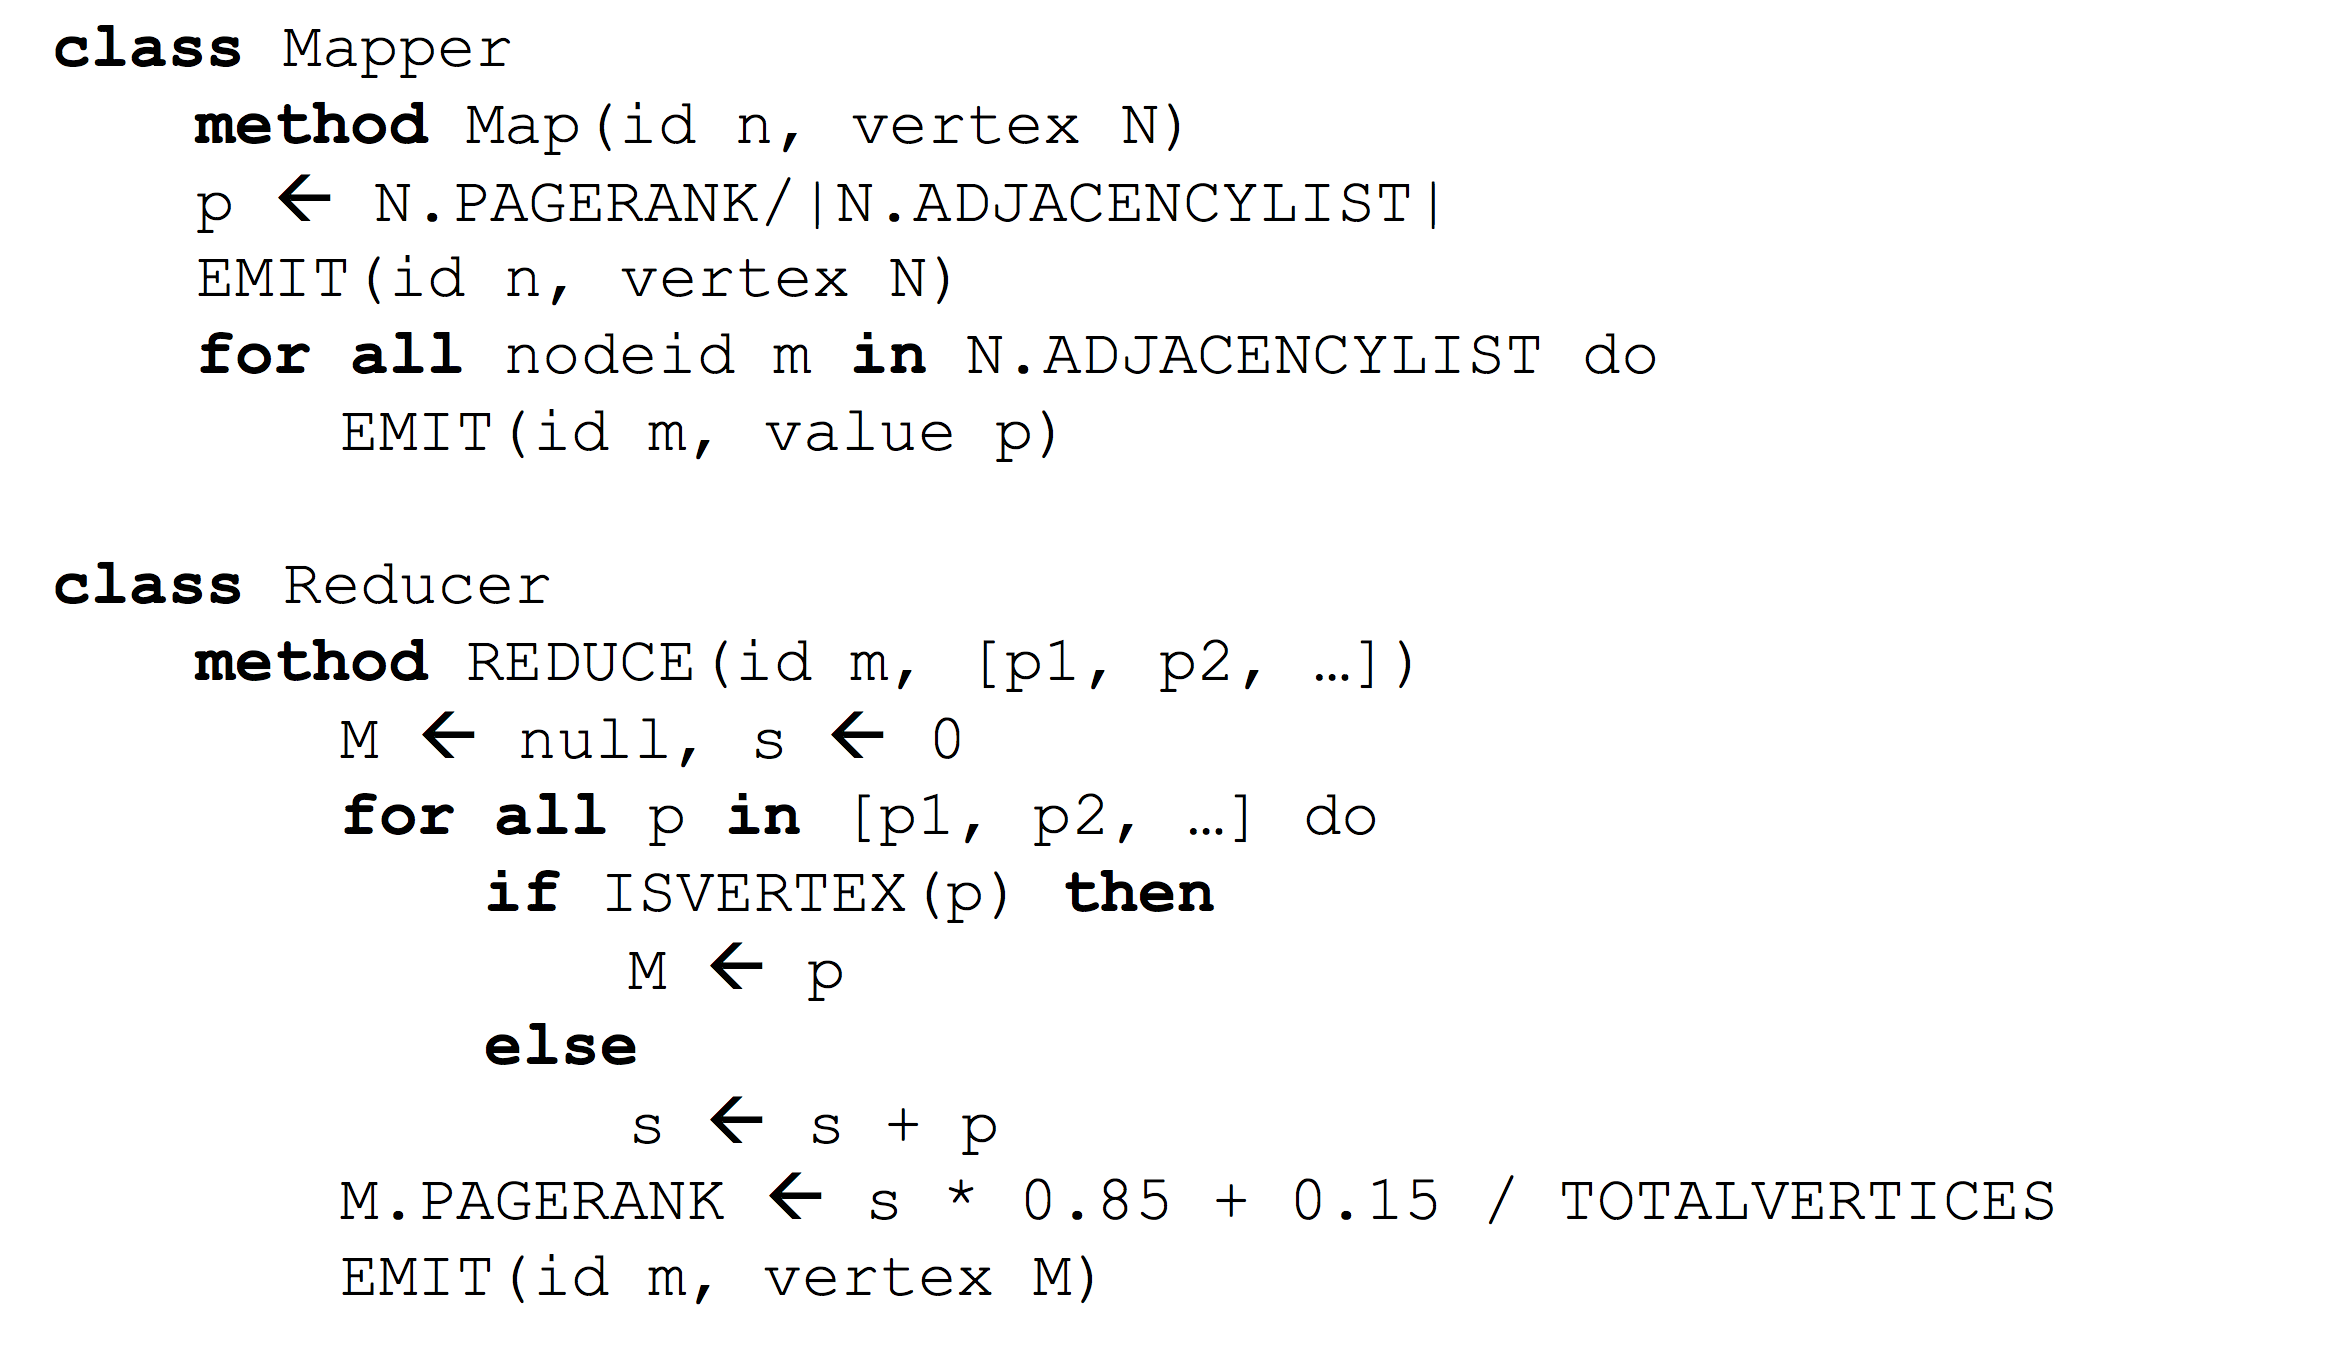
\includegraphics[width=0.8\textwidth]{figs/xx/mapreduce.png}

\end{frame}

\begin{frame}{Why Map-Reduce is not a good choice}	

Problems
\BI
\item The entire state of the graph is shuffled on every iteration
\item We only need to shuffle the new rank contributions, not the graph structure
\item Further, we have to control the iteration outside of MapReduce
\EI

\end{frame}

\begin{frame}{Frameworks for Big Graph Analytics}	


The situation after Map-Reduce
\BI
\item Bulk-Synchronous Parallel 
\BI
  \item Pregel (internal to Google)
  \item Hama
  \item Giraph
  \item Mizan
\EI 
\item Graph Lab / GraphChi
\item Spark / GraphX
\item GPS/Blogel
\EI
	
\end{frame}

\subsection{Pregel}
\subsection{GraphLab}



%%%%%%%%%%%%%%%%%%%%%%%%%%%%%%%%%%%%%%%%%%%%%%%%%%%%%%%%%%%%%%%%%%%%%%%%





% \section{Bibliography}
%
% \begin{frame}{Reading material}
%
% \begin{Bib}
% \BI
% \item \bibentry{complex-networks}
% \EI
% \end{Bib}
%
% \invisible{{\tiny
% \bibliographystyle{abbrv}
% \bibliography{../references}
% }}
%
% \end{frame}

\end{document}